\documentclass{ximera}
\input{../../preamble.tex}
\addPrintStyle{../..}
\begin{document}
    \author{Zomercursus KU Leuven}
    \xmtitle{Basisoefeningen complexe getallen}
    % Start inhoud ximera 

\begin{exercise} Bereken volgende uitdrukkingen. Schrijf de complexe getallen in de vorm $a+bi$.

\begin{question} $(4+i) + (1-2i) = \answer[onlineshowanswerbutton]{5-i}$
\begin{oplossing}
Je kan ofwel reëel en imaginair deel van beide complexe getallen bij elkaar optellen om het antwoord te vinden, ofwel in het complexe vlak de vectorsom maken.
\begin{image}[0.5\textwidth]
	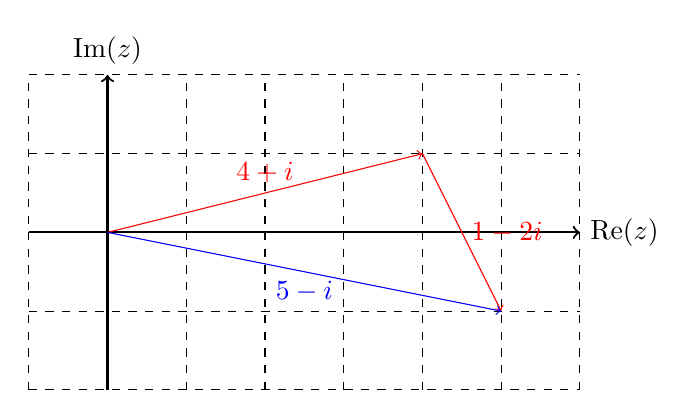
\begin{tikzpicture}[scale=1]
	% grid setup
	
	\def\xmin{-1}
	\def\xmax{6}
	
	\def\ymin{-2}
	\def\ymax{2}				
	
	% grid
	\draw[step = 1.0, black, thin, dashed] (\xmin, \ymin) grid (\xmax, \ymax);
	\draw[->, thick] (\xmin, 0) -- (\xmax, 0) node[right]{Re$(z)$};
	\draw[->, thick] (0, \ymin) -- (0, \ymax) node[above]{Im$(z)$};;	
	
	% tekening
	\draw[->, red]  (0, 0) -- node[above]{$4+i$}  (4,  1);
	\draw[->, red]  (4, 1) -- node[right]{$1-2i$} (5, -1);
	\draw[->, blue] (0, 0) -- node[below]{$5-i$}  (5, -1);	
	\end{tikzpicture}
\end{image}
\end{oplossing}
\end{question}

\begin{question} $ (2+4i) - (6-7i) = \answer[onlineshowanswerbutton]{ -4+11i}$
\begin{oplossing}
Je kan ofwel reëel en imaginair deel van beide complexe getallen bij elkaar optellen om het antwoord te vinden, ofwel in het complexe vlak de vectorsom maken.
\begin{image}[0.5\textwidth]
	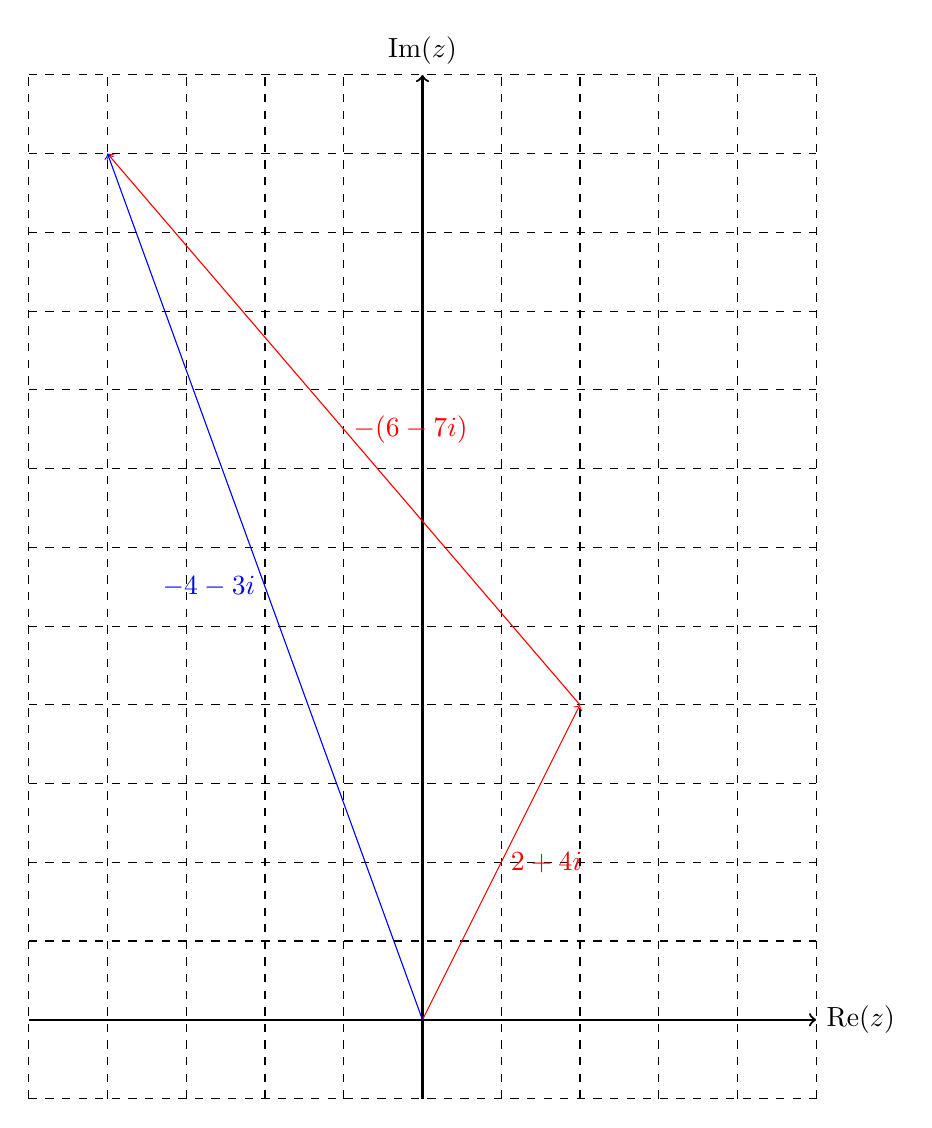
\begin{tikzpicture}[scale=1]
	% grid setup
	
	\def\xmin{-5}
	\def\xmax{5}
	
	\def\ymin{-1}
	\def\ymax{12}				
	
	% grid
	\draw[step = 1.0, black, thin, dashed] (\xmin, \ymin) grid (\xmax, \ymax);
	\draw[->, thick] (\xmin, 0) -- (\xmax, 0) node[right]{Re$(z)$};
	\draw[->, thick] (0, \ymin) -- (0, \ymax) node[above]{Im$(z)$};;	
	
	% tekening
	\draw[->, red]  (0, 0) -- node[right]{$2+4i$}    (2,  4);
	\draw[->, red]  (2, 4) -- node[right]{$-(6-7i)$} (-4, 11);
	\draw[->, blue] (0, 0) -- node[left]{$-4-3i$}   (-4, 11);	
	\end{tikzpicture}
\end{image}
\end{oplossing}
\end{question}

\begin{question} $(2+3i)(-5+i) = \answer[onlineshowanswerbutton]{-13-13i}$
\begin{oplossing}
$$
(2+3i)(-5+i) = -5 + 2i + 3i\cdot(-5) 3i\cdot i = -13 - 13i
$$
\begin{image}[0.5\textwidth]
	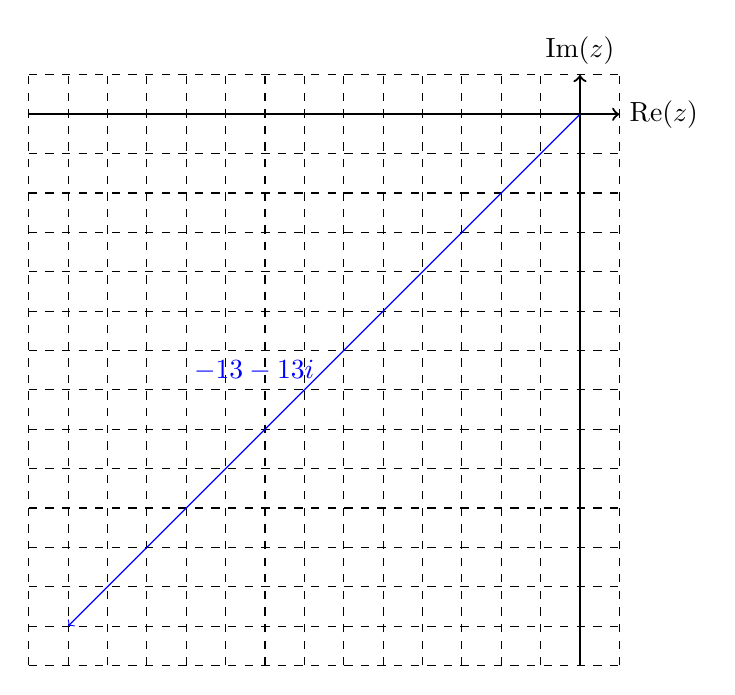
\begin{tikzpicture}[scale=0.5]
	% grid setup
	
	\def\xmin{-14}
	\def\xmax{1}
	
	\def\ymin{-14}
	\def\ymax{1}				
	
	% grid
	\draw[step = 1.0, black, thin, dashed] (\xmin, \ymin) grid (\xmax, \ymax);
	\draw[->, thick] (\xmin, 0) -- (\xmax, 0) node[right]{Re$(z)$};
	\draw[->, thick] (0, \ymin) -- (0, \ymax) node[above]{Im$(z)$};;	
	
	% tekening
	\draw[->, blue] (0, 0) -- node[left]{$-13-13i$}    (-13, -13);	
	\end{tikzpicture}
\end{image}
\end{oplossing}
\end{question}

\begin{question} $(2+i)^2 = \answer[onlineshowanswerbutton]{3+4i}$
\begin{hint}
$(a+b)^2 = a^2 + 2ab + b^2$
\end{hint}
\begin{oplossing}
$$
(2+i)^2  = 4 + 4i + i^2 = 3 + 4i
$$
\begin{image}[0.5\textwidth]
	\begin{tikzpicture}[scale=1.3]
	% grid setup
	
	\def\xmin{0}
	\def\xmax{4}
	
	\def\ymin{0}
	\def\ymax{5}				
	
	% grid
	\draw[step = 1.0, black, thin, dashed] (\xmin, \ymin) grid (\xmax, \ymax);
	\draw[->, thick] (\xmin, 0) -- (\xmax, 0) node[right]{Re$(z)$};
	\draw[->, thick] (0, \ymin) -- (0, \ymax) node[above]{Im$(z)$};;	
	
	% tekening
	\draw[->, blue] (0, 0) -- (3, 4) node[above]{$3+4i$};	
	\end{tikzpicture}
\end{image}
\end{oplossing}
\end{question}

\begin{question} $(2+i)+\overline{(3+2i)} = \answer[onlineshowanswerbutton]{5-i}$
\begin{oplossing}
Merk op dat $\overline{3+2i} = 3-2i$. Dus moeten we de som $(2+i)+ (3-2i)$ bepalen. Je kan ofwel reëel en imaginair deel van beide complexe getallen bij elkaar optellen om het antwoord te vinden, ofwel in het complexe vlak de vectorsom maken.
\begin{image}[0.5\textwidth]
	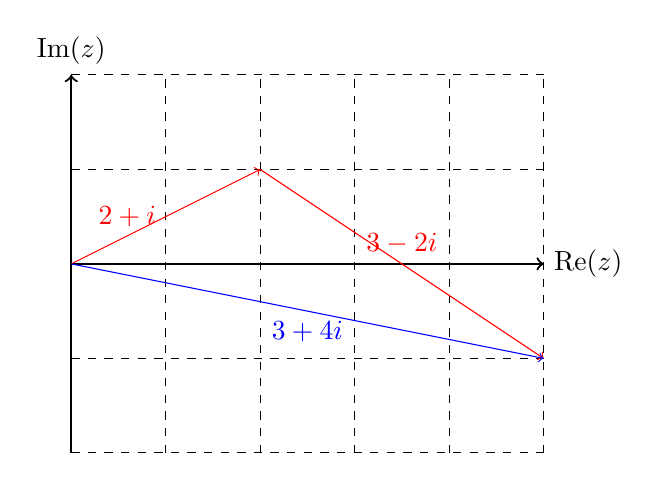
\begin{tikzpicture}[scale=1.2]
	% grid setup
	
	\def\xmin{0}
	\def\xmax{5}
	
	\def\ymin{-2}
	\def\ymax{2}				
	
	% grid
	\draw[step = 1.0, black, thin, dashed] (\xmin, \ymin) grid (\xmax, \ymax);
	\draw[->, thick] (\xmin, 0) -- (\xmax, 0) node[right]{Re$(z)$};
	\draw[->, thick] (0, \ymin) -- (0, \ymax) node[above]{Im$(z)$};;	
	
	% tekening
	\draw[->, red]  (0, 0) -- node[left]{$2+i$}   (2,  1);	
	\draw[->, red]  (2, 1) -- node[above]{$3-2i$} (5, -1);			
	\draw[->, blue] (0, 0) -- node[below]{$3+4i$} (5, -1);	
	\end{tikzpicture}
\end{image}
\end{oplossing}
\end{question}

\begin{question} $(5-6i)(5+6i) = \answer[onlineshowanswerbutton]{61}$
\begin{oplossing}
Je kan de rekenregel $z\cdot \overline{z} = |z|^2$ gebruiken. Dan is $(5-6i)(5+6i) = 25 + 36 = 61$.
\end{oplossing}
\end{question}

\begin{question} $|3-2i| = \answer[onlineshowanswerbutton]{\sqrt{13}}$
\begin{oplossing}
$|3-2i| = \sqrt{3^2 + 2^2} = \sqrt{13}$ 
\end{oplossing}
\end{question}

\begin{question} $|3-2i + \overline {4-2i}| = \answer[onlineshowanswerbutton]{7}$
\begin{oplossing}
Merk eerst op dat $\overline{4-2i} = 4 + 2i$. Je kan ofwel reëel en imaginair deel van beide complexe getallen bij elkaar optellen om de som van twee complexe getallen te vinden, ofwel in het complexe vlak de vectorsom maken.
\begin{image}[0.5\textwidth]
	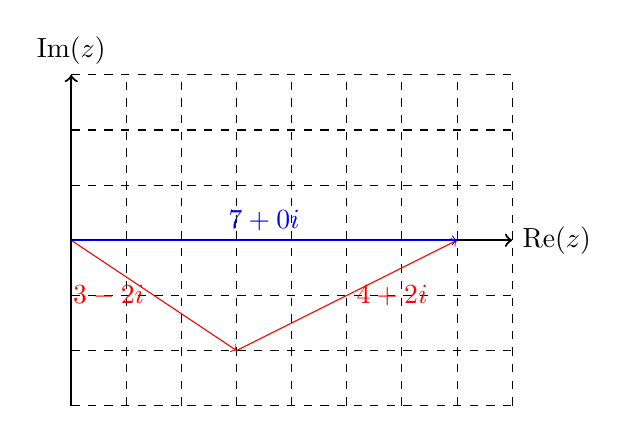
\begin{tikzpicture}[scale=0.7]
	% grid setup
	
	\def\xmin{0}
	\def\xmax{8}
	
	\def\ymin{-3}
	\def\ymax{3}				
	
	% grid
	\draw[step = 1.0, black, thin, dashed] (\xmin, \ymin) grid (\xmax, \ymax);
	\draw[->, thick] (\xmin, 0) -- (\xmax, 0) node[right]{Re$(z)$};
	\draw[->, thick] (0, \ymin) -- (0, \ymax) node[above]{Im$(z)$};;	
	
	% tekening
	\draw[->, red]  (0, 0)  -- node[left]{$3-2i$}  (3,  -2);	
	\draw[->, red]  (3, -2) -- node[right]{$4+2i$}  (7, 0);			
	\draw[->, blue] (0, 0)  -- node[above]{$7+0i$}  (7, 0);	
	\end{tikzpicture}
\end{image}
% Aangezien het resultaat een reëel getal is, is de norm van dit getal hetzelfde als de absolute waarde van dit getal, en $|7|= 7$.
\end{oplossing}
\end{question}

\begin{question} $|3+4i+4+3i|     = \answer[onlineshowanswerbutton]{7\sqrt 2}$
\begin{oplossing}
$|3+4i+4+3i| = |7 + 7i| = \sqrt{49 + 49} = 7 \sqrt{2}$.
\end{oplossing}
\end{question}

\begin{question} $|3+4i|+|4+3i| = \answer[onlineshowanswerbutton]{10}$
\begin{oplossing}
$|3 + 4i| = \sqrt{3^2 + 4^2} = 5$\\
$|4+3i| = \sqrt{4^2 + 3^2} = 5$
\end{oplossing}
\end{question}

\begin{question} $\left| \frac{(3+4i)(-1+2i)}{(-1-i)(3-i)} \right| =  \answer[onlineshowanswerbutton]{\frac52}$
	\end{question}

\end{exercise}
	

\begin{exercise}
	%\id{201206wis08*}
	Een complex getal $z$ kunnen we schrijven als $z=a+bi$ met $a$ en $b$ reële getallen en $i^2=-1$. Dan zijn er onder de lijst van complexe getallen
	\[ 
	\frac{(1+i)^4}{4}, \quad \frac{(1-i)^4}{4}, \quad\frac{(1+i)^2}{2},\quad \frac{(1-i)^2}{2}, \quad i^2 
	\] 
	precies \wordChoice{\choice{$0$}\choice{$1$}\choice{$2$}\choice[correct]{$3$}\choice{$4$}\choice{$5$}\choice{$42$}} die gelijk zijn aan -1. 

\begin{oplossing}
Er is al minstens één van deze complexe getallen gelijk aan -1: de laatste, $i^2$, per definitie van de imaginaire eenheid. 

Je kan best te werk gaan door de derde en vierde uitdrukking te bepalen: de eerste twee complexe getallen zijn hun kwadraten. Hiervoor maken we de volgende berekeningen:
\begin{align*}
	(1+i)^2 &= 1 + 2i + i^2 = 2i  \\
	(1-i)^2 &= 1 - 2i + i^2 = -2i  \\	
\end{align*}
en dus vinden we dat
\begin{align*}
	\frac{(1+i)^2}{2} &= i  \\
	\frac{(1-i)^2}{2} &= -i  \\	
\end{align*}
Het derde en vierde complexe getal zijn dus niet gelijk aan -1. Hun kwadraten zijn echter wel gelijk aan -1: drie van de complexe getallen zijn dus gelijk aan -1. 
\end{oplossing}	
\end{exercise}

\begin{exercise}
	Schets in het complexe vlak de gebieden omschreven door volgende vergelijkingen:

\begin{question} 
$|z| < 1$
\begin{oplossing} $|z|$ is de afstand van $z$ tot de oorsprong. Alle complexe getallen waarvan de afstand tot de oorsprong kleiner is dan 1 liggen \textit{binnen} een cirkel met straal 1, de rand zelf wordt dus niet meegerekend:
           
\begin{image}[0.4\textwidth]
\begin{tikzpicture}[scale=1.4, baseline=(current bounding box.north)]

	\draw[->] (-1.2,0) -- (1.2,0) node[right] {Re$(z)$};
	\draw[->] (0,-1.2) -- (0,1.2) node[above] {Im$(z)$};

	\draw[white, pattern=north west lines, pattern color=blue] (0,0) circle (1cm);
\end{tikzpicture}
\end{image}           
\end{oplossing}
\end{question}

\begin{question} 
$|z| \leq 1$
\begin{oplossing} $|z|$ is de afstand van $z$ tot de oorsprong. Alle complexe getallen waarvan de afstand tot de oorsprong kleiner is dan of gelijk is aan 1 liggen \textit{binnen} een cirkel met straal 1 waarbij de rand zelf wordt meegerekend:
           
\begin{image}[0.4\textwidth]
\begin{tikzpicture}[scale=1.4, baseline=(current bounding box.north)]

	\draw[->] (-1.2,0) -- (1.2,0) node[right] {Re$(z)$};
	\draw[->] (0,-1.2) -- (0,1.2) node[above] {Im$(z)$};

	\draw[blue, thick, pattern=north west lines, pattern color=blue] (0,0) circle (1cm);
\end{tikzpicture}
\end{image}           
\end{oplossing}
\end{question}

\begin{question} 
$|z| = 1$
\begin{oplossing} $|z|$ is de afstand van $z$ tot de oorsprong. Alle complexe getallen waarvan de afstand tot de oorsprong gelijk is aan 1 liggen dus op een cirkel met straal 1:
           
\begin{image}[0.4\textwidth]
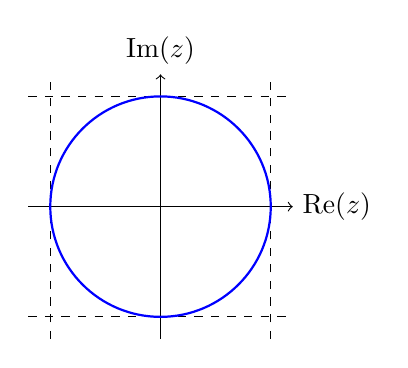
\begin{tikzpicture}[scale=1.4, baseline=(current bounding box.north)]

	\draw[dashed, thin] (-1.2,-1.2) grid (1.2, 1.2);
	\draw[->] (-1.2,0) -- (1.2,0) node[right] {Re$(z)$};
	\draw[->] (0,-1.2) -- (0,1.2) node[above] {Im$(z)$};

	\draw[blue, thick] (0,0) circle (1cm);
\end{tikzpicture}
\end{image}           
\end{oplossing}
\end{question}
            
\begin{question} 
$|z-i| < 1$
\begin{oplossing} 
Alle complexe getallen waarvoor $|z-i| < 1$ zijn alle complexe getallen $z$ waarvoor de afstand tot $i$ kleiner is dan 1:

\begin{image}[0.4\textwidth]
\begin{tikzpicture}[scale=1.4, baseline=(current bounding box.north)]

	\draw[dashed, thin] (-1.2,-1.2) grid (1.2, 2.2);
	\draw[->] (-1.2, 0) -- (1.2, 0) node[right] {Re$(z)$};
	\draw[->] (0, -1.2) -- (0, 2.2) node[above] {Im$(z)$};

	\draw[white, pattern=north west lines, pattern color=blue] (0,1) circle (1cm);	
    \draw (0,1) node[name=Zi,circle, fill=black, radius=1pt,scale=0.5] {} node [fill=white,xshift=-2pt,left] {$i$};   	
\end{tikzpicture}
\end{image}  
\end{oplossing}
\end{question}

\begin{question} 
$|z-i| \geq 1$
\begin{oplossing} Alle complexe getallen waarvoor $|z-i| \geq 1$ zijn alle complexe getallen $z$ waarvoor de afstand tot $i$ groter of gelijk is aan 1: 
\begin{image}[0.4\textwidth]
\begin{tikzpicture}[scale=1.2, baseline=(current bounding box.north)]

	\draw[->] (-2.2, 0) -- (2.2, 0) node[right] {Re$(z)$};
	\draw[->] (0, -1.2) -- (0, 2.2) node[above] {Im$(z)$};
    \draw[pattern=north west lines, pattern color=blue] (-2.2, -1.2) rectangle (2.2, 2.2);
    
	\fill[white] (0,1) circle (1cm);
	\draw[blue, thick] (0,1) circle (1cm);		    
	\draw (0,1) node[name=Zi,circle, fill=black, radius=1pt,scale=0.5] {} node [fill=white,xshift=-2pt,left] {$i$};
\end{tikzpicture}
\end{image}            
\end{oplossing}
\end{question}
			
\begin{question} 
$1 < |z+2i-1| \leq 2$
\begin{oplossing} $1 < |z+2i-1| \leq 2$ kunnen we herschrijven als $1 < |z-(1-2i)| \leq 2$. Alle complexe getallen waarvoor $1 < |z+2i-1| \leq 2$ zijn alle complexe getallen $z$ waarvoor de afstand tot $(1-2i)$ groter is dan 1 en kleiner of gelijk is aan 2:

\begin{image}[0.4\textwidth]
\begin{tikzpicture}[scale=1.2, baseline=(current bounding box.north)]

	\draw[dashed] (-1.2, -4.2) grid (3.2, 1.2);
	\draw[->] (-1.2, 0) -- (3.2, 0) node[right] {Re$(z)$};
	\draw[->] (0, -4.2) -- (0, 1.2) node[above] {Im$(z)$};

	\draw[blue, thick ,pattern=north west lines, pattern color=blue] (1,-2) circle (2);	
	\fill[white] (1,-2) circle (1);
	\draw (1,-2) node[name=Zi,circle, fill=black, radius=1pt,scale=0.5] {} node [fill=white,xshift=3pt,right] {$1-2i$};
\end{tikzpicture}
\end{image}
\end{oplossing}
\end{question}


\begin{question} 
$-1 \leq \text{Im}(z) \leq 2$
\begin{oplossing} Deze ongelijkheden bepalen een \textit{horizontale} strook, aangezien het imaginaire deel van het complex getal in een interval moet liggen. De randen van de strook behoren tot het geschetste domein.

\begin{image}[0.5\textwidth]
\begin{tikzpicture}[scale=0.8, baseline=(current bounding box.north)]
	\draw[dashed] (-5, -2) grid (5, 3);
		
	\draw[->, thick] (-5, 0) -- (5, 0) node[right] {Re$(z)$};
	\draw[->, thick] (0, -2) -- (0, 3) node[above] {Im$(z)$};

	\draw[white, pattern=north west lines, pattern color=blue] (-5,2) rectangle (5, -1);
	
	% randen toevoegen voor duidelijkheid 
	\draw[blue, thick] (-5, -1) -- (5, -1);
	\draw[blue, thick] (-5, 2) -- (5, 2);
\end{tikzpicture}
\end{image}
\end{oplossing}            
\end{question}  


                
\begin{question} 
$|\text{Im}(z)-i| < \sqrt{2}$
\begin{oplossing} Als $z=a+bi$, dan betekent $|\text{Im}(z) - i| < \sqrt{2} $ dat $|b-i| < \sqrt{2}$. Wegens de definitie van modulus is $|b-i|= \sqrt{b^2 + (-1)^2}$. De ongelijkheid wordt dus $\sqrt{b^2 + 1} < \sqrt{2}$, en kwadrateren geeft dan de voorwaarde $b^2 + 1 < 2$ ofwel $b^2 < 1$. Aangezien $b = \text{Im}(z)$, is dit gebied precies de horizontale strook $-1 < \text{Im}(z) < 1$. Merk op dat dit symmetrisch is rond de $x$-as. 

\begin{image}[0.5\textwidth]
\begin{tikzpicture}[scale=0.7, baseline=(current bounding box.north)]
	\draw[dashed] (-5, -2) grid (5, 2);
		
	\draw[->, thick] (-5, 0) -- (5, 0) node[right] {Re$(z)$};
	\draw[->, thick] (0, -2) -- (0, 2) node[above] {Im$(z)$};

	\draw[white, pattern=north west lines, pattern color=blue] (-5,-1) rectangle (5, 1);
\end{tikzpicture}
\end{image}
\end{oplossing}            
\end{question}

\begin{question} 
$|\text{Re}(z)-i| < \sqrt{2}$
\begin{oplossing} 
Als $z=a+bi$, dan betekent $|\text{Re}(z) - i| < \sqrt{2} $ dat $|a-i|<\sqrt{2}$. De berekening van de modulus geeft $\sqrt{a^2 +(-1)^2}< \sqrt{2}$. Na kwadrateren geeft dit $a^2+1 < 2$ of dus $-1 < a < 1$. Aangezien $\text{Re}(z) = a$, is dit gebied precies de verticale strook $-1 < \text{Re}(z) < 1$. Merk op dat dit symmetrisch is rond de $y$-as.
            
\begin{image}[0.4\textwidth]
\begin{tikzpicture}[scale=1.1, baseline=(current bounding box.north)]
	\draw[dashed] (-2, -3) grid (2, 3);
		
	\draw[->, thick] (-2, 0) -- (2, 0) node[right] {Re$(z)$};
	\draw[->, thick] (0, -3) -- (0, 3) node[above] {Im$(z)$};

	\draw[white, pattern=north west lines, pattern color=blue] (-1,3) rectangle (1, -3);
\end{tikzpicture}
\end{image}
\end{oplossing}
\end{question}

\begin{question} 
$\text{Re}(z)> \text{Im}(z)>0$
\begin{oplossing} 
Als $z=a+bi$, dan betekent $\text{Re}(z) > \text{Im}(z) > 0$ dat $a > b > 0$. Dit is het gebied onder de rechte $y = x$, (daar is $a > b$), en boven de $x$-as (daar is $b > 0$):
    
\begin{image}[0.4\textwidth]
\begin{tikzpicture}[scale=1.1, baseline=(current bounding box.north)]
	\draw[dashed] (-0.5, -0.5) grid (2.9, 2.9);
		
	\draw[->, thick] (-0.5, 0) -- (2.9, 0) node[right] {Re$(z)$};
	\draw[->, thick] (0, -0.5) -- (0, 2.9) node[above] {Im$(z)$};
	
	 \draw[white, pattern=north west lines, pattern color=blue] (0,0.02) -- (2.9, 2.9) -- (2.9, 0.02) -- cycle;
\end{tikzpicture}
\end{image}       
\end{oplossing}
\end{question}

% idee: nog een extra oefening van hetzelfde type als hierboven


%%%		niet zo nuttig:

%			\begin{question} 
%				%$\left \{ x+iy \in \C |\;\; y>2x+1 \right \}$
%				Alle $z=x+iy$ die voldoen aan $y>2x+1$
%           \begin{oplossing} De voorwaarde $y>2x+1$ geeft het halfvlak boven de rechte de $y=2x+1$:
%           
%            \tikz[scale=1.2, baseline=(current bounding box.north)]{
%
%                        \draw[white, pattern=north west lines, pattern color=blue] (-1.2,-1.4) -- (1,3)
%                         -- (-1.2,3) -- cycle;
%                        \draw[->] (-1.2,0) -- (2.2,0) node[above] {Re$(z)$};
%                        \draw[->] (0,-1.2) -- (0,3)   node[fill=white,right] {Im$(z)$};
%
%
%            }
%            \end{oplossing}
%            
%            \end{question}

%\end{xmmulticols}
\end{exercise}

\begin{exercise}
Voer volgende delingen uit door de opgave te schrijven in de vorm $a+bi$.

\begin{question}$ \frac{7}{i} = \answer[onlineshowanswerbutton]{-7i}$
\begin{oplossing}
We vermenigvuldigen teller en noemer met $\overline{i} = -i$. In de noemer krijgen we dan $i\cdot (-i) = 1$. Het resultaat is $-7i$. Voor oefeningen kan het handig zijn om te onthouden dat \textit{delen door $i$ hetzelfde is als vermenigvuldigen met $-i$}. % IDEE: dit laatste misschien ook eens bespreken en duidelijk maken in theorie blokje? 
\end{oplossing}
\end{question}
	
\begin{question}$ \frac{1}{5+2i} = \answer[onlineshowanswerbutton]{\frac{5}{29}-\frac{2}{29}i}$
\begin{oplossing}
We vermenigvuldigen teller en noemer met $\overline{5+2i} = 5-2i$. In de noemer krijgen we dan $(5+2i)(5-2i) = 29$.
$$
\frac{1}{5+2i} = \frac{1}{5+2i} \frac{5-2i}{5-2i} = \frac{5-2i}{25}=\frac{5}{29}-\frac{2}{29}i
$$
\end{oplossing}
\end{question}

\begin{question} $ \frac{1+i}{2+3i}	= \answer[onlineshowanswerbutton]{\frac{5}{13}-\frac{1}{13}i}$
\begin{oplossing}
We vermenigvuldigen teller en noemer met $\overline{2+3i} = 2-3i$. In de noemer krijgen we dan $(2+3i)(2-3i) = 13$.
$$
\frac{1+i}{2+3i} = \frac{1+i}{2+3i} \cdot \frac{2-3i}{2-3i} = \frac{5-i}{13}=\frac{5}{13}-\frac{1}{13}i
$$
\end{oplossing}
\end{question}


\begin{question} $ \frac{1+2i}{3-4i} + \frac{2-i}{5i} = \answer[onlineshowanswerbutton]{-\frac{2}{5}}$
\begin{oplossing}
We berekenen de beide termen apart, en tellen de resultaten vervolgens bij elkaar op.

Voor de eerste term: we vermenigvuldigen teller en noemer met $\overline{3-4i} = 3+4i$. In de noemer krijgen we dan $(3-4i)(3+4i) = 25$. De eerste term kunnen we dus vereenvoudigen tot
$$
\frac{1+2i}{3-4i} = \frac{1+2i}{3-4i} \cdot \frac{3+4i}{3+4i} = \frac{-5+10i}{25} = \frac{-1+2i}{5}
$$

Voor de tweede term: we vermenigvuldigen teller en noemer met $\overline{5i} = -5i$. In de noemer krijgen we dan $(5i)\cdot(-5i) = 25$. De tweede term kunnen we dus vereenvoudigen tot
$$
\frac{2-i}{5i} = \frac{2-i}{5i} \cdot \frac{-5i}{-5i} = \frac{-1-2i}{5}
$$
Een andere mogelijkheid is om te gebruiken dat delen door $i$ hetzelfde is als vermenigvuldigen met $-i$, zodat we meteen bekomen dat
$$
\frac{2-i}{5i} = \frac{(2-i)\cdot (-i)}{5} = \frac{-1-2i}{5}
$$

Wanneer we deze twee termen bij elkaar optellen, valt het imaginaire deel weg. Het resultaat is $\frac{-2}{5}$. 
\end{oplossing}
\end{question}
\end{exercise}


%\xmsubsection{Veeltermvergelijkingen}

\begin{exercise}
Bepaal alle oplossingen van volgende veeltermvergelijkingen.



\begin{question}
$ x^2 + x = 0$
\begin{oplossing}
De oplossingen zijn $x_1 = 0$ en $x_2 = -1$.

 We kunnen een $x$ afzonderen in deze vergelijking en vinden dan de equivalente vergelijking $x(x+1) = 0$. Deze heeft als oplossingen $x=0$ en $x=-1$.
\end{oplossing}
\end{question}

\begin{question}
$ x^3 + 16x = 0$
\begin{oplossing}
De oplossingen zijn $x_1 = 0$, $x_2 = 4i$ en $x_3 = -4i$.

 We kunnen een $x$ afzonderen, en vinden dan de equivalente vergelijking $x(x^2+16)=0$. Deze heeft als oplossingen ofwel $x=0$ ofwel $x^2 + 16 = 0$. De laatste vergelijking heeft als oplossingen $x=4i$ en $x=-4i$.
\end{oplossing}
\end{question}


\begin{question}
$ x^2 + 5x + 2 = 0$
\begin{oplossing}
De oplossingen zijn $x_1 = \frac{-5 + \sqrt{17}}{2}$ en $x_2 = \frac{-5 - \sqrt{17}}{2}$.

De vergelijking is van de vorm $ax^2 + bx + c = 0$, met $a=1$, $b=5$ en $c=2$. Dan is $D = b^2 - 4ac = 25-8 = 17$. Omdat $D > 0$, zijn er twee reële oplossingen:
$$
x_1 = \frac{-b + \sqrt{D}}{2a} = \frac{-5 + \sqrt{17}}{2}, \ \ x_2 = \frac{-b - \sqrt{D}}{2a} = \frac{-5 - \sqrt{17}}{2} \, .
$$
\end{oplossing}
\end{question}

\begin{question}
$ x^2 + 4x + 5 = 0$
\begin{oplossing}
De oplossingen zijn $x_1 = -2 - i$ en $x_2 = -2 + i$.

 De vergelijking is van de vorm $ax^2 + bx + c = 0$, met $a=1$, $b=4$ en $c=5$. Dan is $D = b^2 - 4ac = 16 - 20 = -4$. Omdat $D < 0$, zijn er twee complexe oplossingen. De oplossingen zijn
$$
x_1 = \frac{-b + i\sqrt{-D}}{2a} = \frac{-4 + 2i}{2} = -2 + i, \ \ x_2 = \frac{-b - i\sqrt{-D}}{2a} = \frac{-4 - 2i}{2} = -2 - i \, .
$$
\end{oplossing}
\end{question}




\begin{question}
$ 9x^2 - 14 = 4x$
\begin{oplossing}
De oplossingen zijn $x_1 = \frac{2 + \sqrt{130}}{9}$ en $x_2 = \frac{2 - \sqrt{130}}{9}$.

De vergelijking is van de vorm $ax^2 + bx + c = 0$, met $a=9$, $b=-4$ en $c=-14$. Dan is $D = b^2 - 4ac = 16 + 504 = 520$. Omdat $D > 0$, zijn er twee verschillende reële oplossingen. Merk op dat $\sqrt{D} = \sqrt{520} = \sqrt{4 \cdot 130} = 2 \sqrt{130}$. De oplossingen zijn
$$
x_1 = \frac{-b + \sqrt{D}}{2a} = \frac{4 + 2 \sqrt{130}}{18} = \frac{2 + \sqrt{130}}{9}, \ \ x_2 = \frac{-b - \sqrt{D}}{2a} = \frac{4 - 2 \sqrt{130}}{18} = \frac{2 - \sqrt{130}}{9}\, .
$$
\end{oplossing}
\end{question}

\begin{question}
$ x = 2x^2 + 5$
\begin{oplossing}
De oplossingen zijn $x_1 = \frac{1}{4} + \frac{\sqrt{39}}{4} i$ en $x_2 = \frac{1}{4} - \frac{\sqrt{39}}{4} i$.

 De vergelijking is van de vorm $ax^2 + bx + c = 0$, met $a=2$, $b=-1$ en $c=5$. Dan is $D = b^2 - 4ac = 1 - 40 = -39$. Omdat $D < 0$, zijn er twee complexe oplossingen. De oplossingen zijn
$$
x_1 = \frac{-b + i\sqrt{-D}}{2a} = \frac{1 + \sqrt{39}i}{4} = \frac{1}{4} + \frac{\sqrt{39}}{4} i, \ \ x_2 = \frac{-b - i\sqrt{-D}i}{2a} = \frac{1 - \sqrt{39}i}{4} = \frac{1}{4} - \frac{\sqrt{39}}{4} i \, .
$$
\end{oplossing}
\end{question}
% eventueel meer vragen die hogere graden (hoger dan 2) bevatten, zoals in het begin, maar dan iets meer uitdagend
\end{exercise}

\begin{exercise}
Geef een vierkantsvergelijking van de vorm $ax^2 + bx + c = 0$ die
\begin{question}
enkel het getal -5 als oplossing heeft.
\begin{oplossing}
De enige oplossing moet $x = -5$ zijn. Hieruit halen we $x + 5 = 0$, maar dit is geen tweedegraadsvergelijking: $(x+5)^2 = 0$ is dat wel. Voluit geschreven is dit de vergelijking $x^2 +10 x + 25 = 0$. Je kan eventueel met de discriminantmethode nagaan dat $D = 0$ en $\frac{-b}{2a} = -5$.

(Met deze truc kan je zelfs een veeltermvergelijking van eender welke graad geven met enkel -5 als oplossing: $(x+5)^n = 0$: ze voluit schrijven is wel wat lastiger)
\end{oplossing}
\end{question}

\begin{question}
$x_1 = 3-i$ en $x_2 = 3+i$ als oplossingen heeft.
%fout
%\begin{oplossing}
%In feite volstaat het om een vergelijking van de vorm $x^2 + bx + c = 0$ te vinden waarvan dit de oplossingen zijn. Inderdaad, als $x_1$ en $x_2$ voldoen aan $ax^2 + bx + c = 0$, dan voldoen ze ook aan $x^2 + \frac{b}{a}x + \frac{c}{a} = 0$. 
%
%De oplossingen zijn complex, dus moet alvast $D < 0$. Meer nog, omdat $\sqrt{D} = \pm i$, is $b^2 - 4ac = -1$. 
%Verder weten we ook dat $\frac{-b}{2a} = 3$, dus $b = -6a$. Zoals eerder uitgelegd mogen we $a = 1$ veronderstellen, zodat $b = -6$. Uit $\sqrt{D} = \pm i$ volgt dat $b^2 - 4ac = -1$. Met $a = 1$ en $b = -6$ vinden we $36 - 4c= -1$, dus $c = - \frac{37}{4}$.
%\end{oplossing}
\begin{hint}De gezochte vierkantsvergelijking is $(x-x_1)(x-x_2)=0$ \end{hint}
\begin{oplossing}
$(x-x_1)(x-x_2)=(x-3+i)(x-3-i)=x^2 -(3+i)x+(-3+i)x+(-3+i)(-3-i)=x^2-6x+10$
\end{oplossing}
\end{question}
\end{exercise}

%\begin{oefening2}
%	Los volgende vergelijkingen in $z\in \C$ op. Schrijf het resultaat in de vorm $a+bi$.
%	\begin{enumerate}
%		\item $5i \;z+2=3i$
%		\item $(3+i)(z+1)=z$
%		\item $\ds{\frac{7}{z+i}=1-i}$
%		\item $3 z +2 \overline z=10-i$
%		\item $(2+i) \; \overline z =z+4$
%	\end{enumerate}
%	\begin{opl}
%		\begin{enumerate}
%			\item $\frac{3}{5} +\frac{2i}{5}$
%			\item $\frac{-7}{5} +\frac{i}{5}$
%			\item $\frac{7}{2} +\frac{5i}{2}$
%			\item $2-i$
%			\item $3+i$
%		\end{enumerate}
%	\end{opl}
%\end{oefening2}
%
%\begin{oefening2}
%	%An Vanfroyenhoven
%	%\id{2015wis01}
%	
%	Veronderstel dat $x$ en $y$ complexe getallen zijn die voldoen aan het stelsel 
%	\begin{equation*}
%	\begin{cases}
%	(-1-i)x-2y & = 4 \\
%	x+(2-i)y   & = i,
%	\end{cases}
%	\end{equation*}
%	waarbij $i^2=-1$.
%	
%	Bepaal $x+y$.
%	\begin{enumerate}
%		\item [(A)] $x+y=-1+4i$
%		\item [(B)] $x+y=-1+2i$
%		\item [(C)] $x+y=-1$
%		\item [(D)] $x+y=1$
%		\item [(E)] $x+y$ kan oneindig veel waarden aannemen.
%	\end{enumerate}
%	
%	\begin{opl}
%		A 
%	\end{opl}
%	
%	\bron{ijkingstoets juli 2015}
%\end{oefening2}
%
%\begin{oefening2}
%	Bereken
%	\[  \left| \frac{(3+4i)(-1+2i)}{(-1-i)(3-i)}\right|\]
%	\begin{opl}
%		$\ds\frac{5}{2}$
%	\end{opl}
%\end{oefening2}
%
%\newpage
%\begin{oefening2}
%	%\id{2013hds05}
%	%\id{201307beg14**}
%	
%	Als het complex getal $z$ voldoet aan
%	$$
%	z^2 = \frac{(2+i)(-1+2i)}{2(3+4i)}
%	$$
%	dan is de modulus van $z$:
%	\begin{enumerate}
%		\item [(A)]$|z| = \frac{1}{2}$
%		\item [(B)] $|z| = \frac{\sqrt{2}}{2}$
%		\item [(C)]$|z| = \sqrt{2}$
%		\item [(D)]$|z| = - \frac{\sqrt{2}}{2}$
%		\item [(E)]$|z| = \frac{1}{4}$
%	\end{enumerate}
%	
%	
%	\begin{opl}
%		B
%	\end{opl}
%	\bron{ijkingstoets juli 2013}
%	
%\end{oefening2}
%
%\begin{oefening2}
%	%\id{SCvraag1}
%	
%	De getallen $\alpha$ en $\beta$ zijn re\"ele getallen, $i^2=-1$. Als $z_1=1-2i$ een nulpunt is van de complexe
%	veelterm $z^2-(\alpha+i)z+(7+i\beta)$,
%	wat is dan het tweede nulpunt $z_2$?
%	
%	\begin{enumerate}
%		\item [(A)] $z_2=1+2i$
%		\item [(B)] $z_2=1+i$
%		\item [(C)] $z_2=3$
%		\item [(D)] $z_2=1+3i$
%		\item [(E)] $z_2=1-3i$
%	\end{enumerate}
%	
%	
%	\begin{opl}
%		D
%	\end{opl}
%	
%	\bron{ijkingstoets juli 2015}
%\end{oefening2}
%
%%%%%%%%%%%%
%
%%%%%%%%%%%
%
%
%
%
%
%
%
%%%%%%%%%%%%%%
%\begin{oefening2}
%	%\id{2015wis09}
%	
%	Het complexe getal $z$ is de oplossing van de vergelijking $(2+i)(z+i)=z-1$, waarbij $i^2=-1$. Bereken de modulus van $z$.
%	
%	\vspace{4mm}
%	
%	(A) $|z|=1$\hspace{1cm}
%	(B) $|z|=\sqrt 2$ \hspace{1cm}
%	(C) $|z|=2$ \newline
%	(D) $|z|=\sqrt 5$  \hspace{1cm}
%	(E) $|z|=2\sqrt 5$
%	
%	
%	\begin{opl}
%		B
%	\end{opl}
%	%
%	%\cat{vaardigheden}
%	%\class{**}
%	%\info{ijkingstoets september 2015 - 313 deelnemers} 
%	%\juist{62} 
%	%\blanco{23} 
%	%\ul{85/36}
%	\bron{ijkingstoets september 2015}
%\end{oefening2}
%%%%%%%%%
%\newpage
%
%\begin{oefening2}
%	Bereken
%	\begin{enumerate} \item  $(-1-i)^{20}$
%		\item $(1+i)^{21}$
%		\item $(-\sqrt{3}+i)^5$
%	\end{enumerate}
%	\begin{opl}\mbox{}
%		\begin{enumerate}
%			\item $-1024$
%			\item $-1024-1024i$
%			\item $16\sqrt{3}+16i$
%		\end{enumerate}
%	\end{opl}
%\end{oefening2}
%
%\begin{oefening2}
%	Los op in $\C$ en geef de ontbinding in factoren.
%	\begin{enumerate}
%		\item $-x^2+x-2=0\qquad$
%		\item  $ 2x^2-10x+13=0\qquad$
%		\item  $ 3x^2-5x+7=0\qquad$
%	\end{enumerate}
%	
%	\begin{opl}
%		\begin{enumerate}
%			\item $x_{1,2}=\frac{1\pm i \sqrt{7} }{2}$, de ontbinding is
%			$-x^2+x-2=-1(x-\frac{1+ i \sqrt{7}}{2})(x-\frac{1- i
%				\sqrt{7}}{2})$
%			\item $x_{1,2}=\frac{5\pm i}{2}$, de ontbinding is
%			$2x^2-10x+13=2(x-\frac{5+ i}{2})(x-\frac{5-i}{2})$
%			\item $x_{1,2}=\frac{5\pm i \sqrt{59} }{6}$, de ontbinding is
%			$3x^2-5x+7=3(x-\frac{5+ i \sqrt{59} }{6})(x-\frac{5- i \sqrt{59}
%			}{6})$
%		\end{enumerate}
%	\end{opl}
%\end{oefening2}
%
%\begin{oefening2}
%	Zoek een vierkantsvergelijking met re\"ele co\"effici\"enten
%	waarvan $3+2i$  een wortel is.
%	\begin{opl}
%		$x^2-6x+13=0$
%	\end{opl}
%\end{oefening2}
%
%\begin{oefening2}
%	Zoek alle complexe wortels van volgende vergelijking
%	$(x^2+5)(x^3+x-2)=0.$
%	\begin{opl}
%		$\pm\sqrt{5}\;i, 1,\ds \frac{-1\pm\sqrt{7}\;i}{2}$
%	\end{opl}
%\end{oefening2}
%
%
%\begin{oefening2}
%	Los de binomiaalvergelijking $z^3=1+i$ op. Stel de
%	oplossingen voor in het complex vlak.
%\end{oefening2}
%
%\begin{oefening2}
%	Beschouw een $z\in\C$ met $|z|=1$.
%	\begin{enumerate}
%		\item Toon aan dat $\left(\ds\frac{1+z}{|1+z|}\right)^2=z.$
%		\item Kan je dat resultaat ook meetkundig verklaren? Teken daartoe
%		$z$ (ergens op de eenheidscirkel), waar ligt dan $1+z$ en $\ds
%		\ds\frac{1+z}{|1+z|}\;\dots$?
%	\end{enumerate}
%\end{oefening2}
%
%




\end{document}
